\documentclass{praktikum}
\usepackage{pgfplots}
\usepackage{graphicx}

%\usepackage{tikzpicture}
%====== Vyplňte údaje ======
%% dobrá rada na začátek - pokud nevíš, co měníš, zálohuj to, co funguje ;)
\def\mydotfill{\unskip\nobreak\leaders\hbox{.}\hskip 4em plus 1fill\relax}
\jmeno{Matyáš Peroutík}
\kod{256371}
\rocnik{1}
\obor{AMT}
\skupina{}
\labskup{B}
\spolupracoval{Štěpán Pavlica}


\ucitel{}
\merenodne{13.\,3.\,2024}
\odevzdanodne{27.\,3.\,2024}

\priprava{}
\opravy{}
\nazev{Tíhové Zrychlení}
\cislo{10} %měřené úlohy



\begin{document}
%====== Vygenerování tabulky ======
\maketitle
\vspace{0.5 cm}

%====== Text protokolu zde ======

\section{Úkol měření}
\paragraph{}
Stanovte lokální tíhové zrychlení pomocí měření reverzním kyvadlem.
\section{Teoretický rozbor}

\subsection{Základní pojmy}

\subsubsection{Tíhové zrychlení \textit{g}} 
\paragraph{}Je zrychlení volného pádu ve vakuu. Jednotkou je $ms^{-2}$. Toto zrychlení je důsledkem hlavně gravitační síly země (Newtonův gravitační zákon) a odstředivé síly země (rotace). Dále na její velikost může působit např. poloha měsíce. Tudíž tíhové zrychlení není konstantní. V Brně je tabulková hodnota tíhového zrychlení \textit{g = 9.813~$ms^{-2}$}.

\subsubsection{Těžiště}
\paragraph{} Je bod tuhého tělěsa, v němž se v homogenním tíhovém poli protínají těžnice. V tomto bodě leží vektor tíhy tělesa.

\subsubsection{Hmotný střed}
\paragraph{} Je bod, který vychází ze tvaru tělesa a rozložení jeho hmoty. Tento bod je možné zapsat matematickými vztahy. V homogenním tíhovém poli splývá s těžištěm.

\subsubsection{Kyvadlo}
\paragraph{} Je libovolné těleso, které se může otáčet kolem pevné vodorovné osy, ktera neprochází těžištěm. Při vychýlení z jeho rovnovážné polohy se těleso začne kývat.


\subsubsection{Fyzické kyvadlo}
\paragraph{} Je kyvadlo, které je pomocí tří podmínek zjednodušeno. Při práci s fyzickým kyvadlem uvažujeme, že je těleso kyvadla tuhé, že se otáčí kolem osy bez tření a při kývaní není zpomalováno vlivem okolí. Doba kmitu (periody) fyzického kyvadla pro rozkyv zhruba do $5^o$ je dána tímto vztahem:

\begin{equation}
\label{eqn:T_fyzicke_kyvadlo}
T = 2 \pi \sqrt{\frac{J}{mg\textit{l}}}
\end{equation}
\textit{J}\mydotfill setrvačnost kyvadla vzhledem k ose kývání\linebreak
\textit{m}\mydotfill hmotnost kyvadla\linebreak
\textit{l}\mydotfill vzdálenost osy kyvu od těžiště kyvadla 

\subsubsection{Matematické kyvadlo}
\paragraph{} Je maximálně zjednodušené kyvadlo. Zkoumá pouze pohyb hmotného bodu na tenkém nedeformovatelném vlákně s hmotností, kterou při výpočtu můžeme zanedbat. Doba kmitu (periody) matematického kyvadla pro rozkyv zhruba do $5^o$ je dána tímto vztahem:

\begin{equation}
\label{eqn:T_matematicke_kyvadlo}
T=2 \pi \sqrt{\frac{l}{g}}
\end{equation}
\textit{l} \mydotfill délka matematického kyvadla\linebreak
\textit{g} \mydotfill tíhové zrychlení

Doba kmitu zde nezávisí na hmotnosti hmotného bodu. Pokud budeme těleso tedy uvažovat za pouhý bod, tak délka l matematického kyvadla je zároveň vzdálenost osy kyvu od těžiště.
\subsection{Teorie měření reverzním kyvadlem}
\paragraph{}
\textbf{Reverzní kyvadlo} je dvouosé fyzické kyvadlo, jehož závaží má nastavitelnou pevnou polohu. Protože se jedná o kyvadlo fyzické, tak je jeho doba kyvu určena vztahem (\ref{eqn:T_fyzicke_kyvadlo}). Tento vztah ale není příliž vhodný pro výpočet tíhového zrychlení, protože většinou neznáme setrvačnost kyvadla \textit{J} a přesnou vzdálenost osy kyvu od těžiště \textit{l}. Proto se snažíme vytvořit podmínky takové, abychom mohli použít vztah pro kyvadlo matematické (\ref{eqn:T_matematicke_kyvadlo}). Pro to alevšak musíme znát redukovanou délku kyvadla \textit{$l_r$}. Při této délce má kyvadlo v obou polohách stejnou dobu kmitu. Pokud ze vztahu (\ref{eqn:T_matematicke_kyvadlo}) vyjádříme tíhové zrychlení, dostaneme pro tíhové zrychlení následující vztah:

\begin{equation}
\label{eqn:g_reverzni_redukovane}
g=\frac{4 \pi ^2 l_r}{T^2}
\end{equation}

Redukovanou délku reverzního kyvadla hledáme tím způsobem, že posouváním závaží měníme dobu periody osy 1 ($T_1$) a osy 2 ($T_2$). Jakmile nalezneme takovou polohu závaží, že se tyto periody rovnají, tak můžeme uvažovat vzdálenost os jako redukovanou délku.

\section{Naměřené hodnoty}

\begin{table}[H]
	\label{tab:namerene_reduk_delka}
    \centering
    \renewcommand{\arraystretch}{2}
    \begin{tabular}{|c|c|c|c|c|c|c|c|c|c|c|}
    \hline
        \parbox{1,5cm}{číslo měření} & 1 & 2 & 3 & 4 & 5 & 6 & 7 & 8 & 9 & 10 \\
        \hline
        $\dfrac{l_r}{cm}$ & 96,45 & 96,50  & 96,55 & 96,50 & 96,40 & 96,50 & 96,45 & 96,55 & 96,50 & 96,50 \\
        \hline
    \end{tabular}
    \caption{Měřené hodnoty délky $l_r$ mezi osami $O_1$ a $O_2$}
    \label{tab:měřené délky}
\end{table}


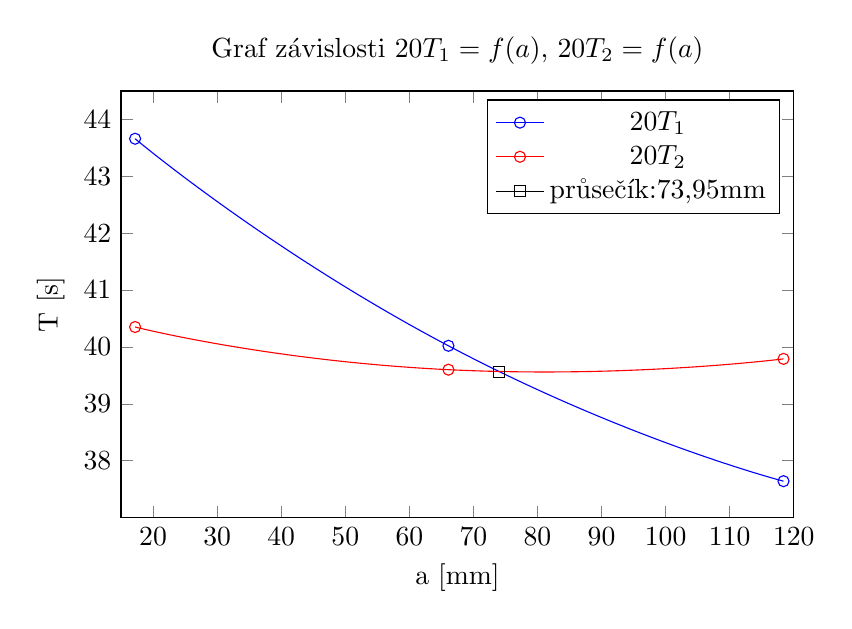
\begin{tikzpicture}

\begin{axis}[
    title={Graf závislosti $20T_1=f(a)$, $20T_2=f(a)$},
    xlabel={a [mm]},
    ylabel={T [s]},
    xmin=15, xmax=120,
    ymin=37, ymax=44.5,
    xtick={20,30,40,50,60,70,80,90,100,110,120},
    ytick={38,39,40,41,42,43,44},
    width=\columnwidth-2cm, height=7cm,
]

\addplot[
    color=blue,
    mark=o,
    smooth, tension=01,
    ]
    coordinates {
    (17.2,43.66)(66.1,40.02)(118.4,37.64)
    };
    \addlegendentry{$20T_1$}

\addplot[
    color=red,
    mark=o,
    smooth, tension=01,
    ]
    coordinates {
    (17.2,40.35)(66.1,39.6)(118.4,39.79)
    };
    \addlegendentry{$20T_2$}

\addplot[
    color=black,
    mark=square,
    ]
    coordinates {
    (73.95,39.56)
    };
    \addlegendentry{průsečík:73,95mm}
    

    
\end{axis}
\end{tikzpicture}


\begin{table}[H]
\begin{adjustbox}{width=\columnwidth,center}
    %\centering
    \renewcommand{\arraystretch}{1.5}
    \begin{tabular}{c c c}
        a [mm] & $20T_1$ [s] & $20T_2$ [s]\\ 
        17,2 & 43,66 & 40,35 \\
        66,1 & 40,02 & 39,60 \\
        118,4 & 37,64 & 39,79 \\
    \end{tabular} \hspace{3cm}
    \begin{tabular}{c c c}
        počet kmitů & $T_1$ [s] & $T_2$ [s]\\
        0 & 0 & 0 \\
        10 & 19,79 & 19,74 \\
        20 & 39,58 & 39,49 \\
        30 & 59,37 & 59,23 \\
        40 & 79,16 & 78,97 \\
        50 & 98,95 & 98,72 \\
        60 & 118,73 & 118,46 \\
        70 & 138,52 & 138,2 \\
        80 & 158,3 & 157,95 \\
        90 & 178,07 & 177,69 \\
    \end{tabular}

    \label{tab:merene}
\end{adjustbox}
\end{table}

\section{Zpracování hodnot}

Nejprve je zpracována hodnota redukované délky. Následně je zpracovány hodnoty tíhového zrychlení pro každou osu zvlášť použítím postupné metody.

\subsection{Redukovaná délka \textit{$l_r$}}

\begin{table}[H]
	\label{tab:vypocet_reduk_delka}
    \centering

    \renewcommand{\arraystretch}{2}
    \resizebox{\columnwidth}{!}{%
    \begin{tabular}{|c|c|c|c|c|c|c|c|c|c|c|}
    \hline
        \parbox{1,5cm}{číslo měření} & 1 & 2 & 3 & 4 & 5 & 6 & 7 & 8 & 9 & 10 \\
        \hline
        $\dfrac{l_r}{cm}$ & 96,45 & 96,50  & 96,55 & 96,50 & 96,40 & 96,50 & 96,45 & 96,55 & 96,50 & 96,50 \\
        \hline
         $(l_i-\overline{l_r})^2$ 
          & $1.6 \cdot 10^{-3}$ 
          & $1 \cdot 10^{-4}$ 
          & $3.6 \cdot 10^{-3}$  
          & $1 \cdot 10^{-4}$ 
          & $8.1 \cdot 10^{-3}$ 
          & $1 \cdot 10^{-4}$ 
          & $1.6 \cdot 10^{-3}$ 
          & $3.6 \cdot 10^{-3}$ 
          & $1 \cdot 10^{-4}$ 
          & $1 \cdot 10^{-4}$  \\
        \hline
    \end{tabular}%
}
    \caption{Zpracování redukované délky $l_r$ }
    \label{tab:měřené délky}
\end{table}

\[ \overline{l_r}=\frac{1}{n}\sum l_i = 96.49 cm \]
\[ s^2 = \frac{\sum (l_i -\overline{l_r})^2}{n-1}\doteq 2.111 \cdot 10^{-3} cm^2 \]
\[ s = \sqrt{\frac{\sum (l_i -\overline{l_r})^2}{n-1}}\doteq 0.04595cm \]
\[  = t_{10;0,95} \cdot \frac{s}{\sqrt{n}} \doteq 0.03371 cm \]
\[ \delta_r(l_r) =\frac{\delta(l_r)}{\overline{l_r}} \doteq 3.494 \cdot 10^{-4} cm \]
\[ l_r = (96.49 \pm 0.03) cm \]

\textbf{Legenda k výpočtům:}\\ \\
\textit{$\overline{l_r}$}\mydotfill průměrná hodnota změřené redukované délky kyvadla\\
\textit{$s^2$}\mydotfill rozptyl změřených hodnot redukované délky\\
\textit{s}\mydotfill směrodatná odchylka změřených hodnot redukované délky\\
\textit{$t_{10;0,95}$} \mydotfill koeficient studentova rozdělení dle tabulky ($t_{10;0,95}$ = 2.32)\\
\textit{$\delta(l_r)$} \mydotfill absolutní chyba výsledku\\
\textit{$\delta_r(l_r)$} \mydotfill relativní chyba výsledku


\subsection{Výpočty pro osu \textit{$O_1$}}


%Please add the following required packages to your document preamble:
% \usepackage{graphicx}
\begin{table}[H]
\centering
\resizebox{0.7\columnwidth}{!}{%
\begin{tabular}{|c|c|c|c|c|}
\hline
\textbf{\begin{tabular}[c]{@{}c@{}}počet\\ kmitů\end{tabular}} &
  \textbf{\begin{tabular}[c]{@{}c@{}}A\\ čas (s)\end{tabular}} &
  \textbf{\begin{tabular}[c]{@{}c@{}}počet\\ kmitů\end{tabular}} &
  \textbf{\begin{tabular}[c]{@{}c@{}}B\\ čas (s)\end{tabular}} &
  \textbf{\begin{tabular}[c]{@{}c@{}}rozdíly sloupců B-A\\ 50T (s)\end{tabular}} \\ \hline
\textit{0T}  & \textit{0}     & \textit{50T} & \textit{98.95}  & \textit{98.95} \\ \hline
\textit{10T} & \textit{19.79} & \textit{60T} & \textit{118.73} & \textit{98.94} \\ \hline
\textit{20T} & \textit{39.58} & \textit{70T} & \textit{138.52} & \textit{98.94} \\ \hline
\textit{30T} & \textit{59.37} & \textit{80T} & \textit{158.30} & \textit{98.93} \\ \hline
\textit{40T} & \textit{79.16} & \textit{90T} & \textit{178.07} & \textit{98.91} \\ \hline
\end{tabular}%
}
\caption{Výpočtová tabulka dob kmitů pomocí postupné metody}
\label{tab:vypocty_osa1}
\end{table}


\[\overline{50T_1} = \frac{1}{n}\sum 50T_i = 98.934s \]
\[s^2 = \frac{\sum (50T_i - \overline{50T_1})^2}{n-1} \doteq 2.3 \cdot 10^{-4} s^2\]
\[s = \sqrt{\frac{\sum (50T_i - \overline{50T_1})^2}{n-1}}\doteq 0.01517 s \]
\[\delta(50T_1) = t_{5;0.95} \cdot \frac{s}{\sqrt{n}} \doteq 2.035 \cdot 10^{-4} \]
\[\delta(50T_1) = \frac{\delta(50T_1)}{\overline{50T_1}} = 2.034 \cdot 10^{-4}\]
\[50T_1 = (98.93 \pm 0.02) s \]
\[T1 = (1.9798 \pm 0.0004) s\]

\textbf{Legenda k výpočtům:}\\ \\
\textit{$\overline{50T_1}$}\mydotfill průměrná hodnota délky 50-ti kmitů osy 1\\
\textit{$s^2$}\mydotfill rozptyl hodnot délky 50-ti kmitů osy 1\\
\textit{s}\mydotfill směrodatná odchylka hodnot délky 50-ti kmitů osy 1\\
\textit{$t_{10;0,95}$} \mydotfill koeficient studentova rozdělení dle tabulky ($t_{5;0,95}$ = 2.968)\\
\textit{$\delta(l_r)$} \mydotfill absolutní chyba výsledku\\
\textit{$\delta_r(l_r)$} \mydotfill relativní chyba výsledku \\
\textit{$50T_1$} \mydotfill delka 50-ti kmitů osy 1\\
\textit{T1} \mydotfill delka jednoho kmitu osy 1
\\ \\
Z těchto hodnot můžeme vypočítat průměrnou hodnotu tíhového zrychlení určené osou~1

\[\overline{g} = \frac{4 \pi ^2 \overline{l_r}}{\overline{T_1}^2} \doteq 9.7265 ms^{-2} \]

a následně určit chybu tíhového zrychlení pomocí derivace vztahu (\ref{eqn:g_reverzni_redukovane}).

\[\delta(g_1) = \sqrt{\left(\frac{\partial g}{\partial l_r}\delta(l_r)\right)^2 +
 \left(\frac{\partial g}{\partial T}\delta(T_1)\right)^2 } = 
\overline{g}\sqrt{\left(\frac{\delta(l)}{\overline{l}}\right)^2+\left(-2\frac{\delta(T_1)}{T_1}\right)^2} \doteq 5.217 \mu s^{-2}
 \]

\[ \delta_r(g_1) = \frac{\delta(g_1)}{\overline{g_1}} \doteq 5.364 \cdot 10^{-4} \] 

\[ g_1 = (9.727 \pm 0.005) ms^{-2} \]

\textbf{Legenda k výpočtům:}\\ \\
\textit{$\delta(g_1)$} \mydotfill absolutní chyba tíhového zrychlení osy 1\\
\textit{$\delta_r(g_1)$} \mydotfill relativní chyba tíhového zrychlení osy 1\\
\textit{$g_1$} \mydotfill tíhové zrychlení osy 1\\


\subsection{Výpočty pro osu \textit{$O_2$}}


% Please add the following required packages to your document preamble:
% \usepackage{graphicx}
\begin{table}[H]
\centering
\resizebox{0.7\columnwidth}{!}{%
\begin{tabular}{|c|c|c|c|c|}
\hline
\textbf{\begin{tabular}[c]{@{}c@{}}počet\\ kmitů\end{tabular}} &
  \textbf{\begin{tabular}[c]{@{}c@{}}A\\ čas (s)\end{tabular}} &
  \textbf{\begin{tabular}[c]{@{}c@{}}počet\\ kmitů\end{tabular}} &
  \textbf{\begin{tabular}[c]{@{}c@{}}B\\ čas (s)\end{tabular}} &
  \textbf{\begin{tabular}[c]{@{}c@{}}rozdíly sloupců B-A\\ 50T (s)\end{tabular}} \\ \hline
\textit{0T}  & \textit{0}     & \textit{50T} & \textit{98.72}  & \textit{98.72} \\ \hline
\textit{10T} & \textit{19.74} & \textit{60T} & \textit{118.46} & \textit{97.72} \\ \hline
\textit{20T} & \textit{39.49} & \textit{70T} & \textit{138.2}  & \textit{98.71} \\ \hline
\textit{30T} & \textit{59.23} & \textit{80T} & \textit{157.95} & \textit{97.72} \\ \hline
\textit{40T} & \textit{78.97} & \textit{90T} & \textit{177.69} & \textit{97.72} \\ \hline
\end{tabular}%
}
\caption{Výpočtová tabulka dob kmitů pomocí postupné metody}
\label{tab:vypocty_osa2}
\end{table}



\[\overline{50T_2} = \frac{1}{n}\sum 50T_i = 98.718s \]
\[s^2 = \frac{\sum (50T_i - \overline{50T_2})^2}{n-1} \doteq 2 \cdot 10^{-5} s^2\]
\[s = \sqrt{\frac{\sum (50T_i - \overline{50T_2})^2}{n-1}}\doteq 4.472 \cdot 10^{-3} s \]
\[\delta(50T_2) = t_{5;0.95} \cdot \frac{s}{\sqrt{n}} \doteq 5.896 \cdot 10^{-3} \]
\[\delta(50T_2) = \frac{\delta(50T_1)}{\overline{50T_1}} = 5.973 \cdot 10^{-5}\]
\[50T_1 = (98.718 \pm 0.006) s \]
\[T1 = (1.97436 \pm 0.00012) s\]

\textbf{Legenda k výpočtům:}\\ \\
\textit{$\overline{50T_2}$}\mydotfill průměrná hodnota délky 50-ti kmitů osy 2\\
\textit{$s^2$}\mydotfill rozptyl hodnot délky 50-ti kmitů osy 2\\
\textit{s}\mydotfill směrodatná odchylka hodnot délky 50-ti kmitů osy 2\\
\textit{$t_{10;0,95}$} \mydotfill koeficient studentova rozdělení dle tabulky ($t_{5;0,95}$ = 2.968)\\
\textit{$\delta(l_r)$} \mydotfill absolutní chyba výsledku\\
\textit{$\delta_r(l_r)$} \mydotfill relativní chyba výsledku \\
\textit{$50T_2$} \mydotfill delka 50-ti kmitů osy 2\\
\textit{T2} \mydotfill delka jednoho kmitu osy 2
\\ \\
Z těchto hodnot můžeme vypočítat průměrnou hodnotu tíhového zrychlení určené osou~1

\[\overline{g} = \frac{4 \pi ^2  \overline{l_r}}{\overline{T_2}^2} \doteq 9.7721 ms^{-2} \]

a následně určit chybu tíhového zrychlení pomocí derivace vztahu (\ref{eqn:g_reverzni_redukovane}).

\[\delta(g_2) = \sqrt{\left(\frac{\partial g}{\partial l_r}\delta(l_r)\right)^2 +
 \left(\frac{\partial g}{\partial T}\delta(T_2)\right)^2 } = 
\overline{g}\sqrt{\left(\frac{\delta(l)}{\overline{l}}\right)^2+\left(-2\frac{\delta(T_2)}{T_2}\right)^2} \doteq 3.608 \mu s^{-2}
 \]

\[ \delta_r(g_2) = \frac{\delta(g_2)}{\overline{g_2}} \doteq 3.692 \cdot 10^{-4} \] 

\[ g_2 = (9.772 \pm 0.004) ms^{-2} \]

\textbf{Legenda k výpočtům:}\\ \\
\textit{$\delta(g_2)$} \mydotfill absolutní chyba tíhového zrychlení osy 2\\
\textit{$\delta_r(g_2)$} \mydotfill relativní chyba tíhového zrychlení osy 2\\
\textit{$g_2$} \mydotfill tíhové zrychlení osy 2\\


\section{Závěr}
\paragraph{}
Porovnáním hodnot tíhových zrychlení v jednotlivých osách, které jsme pomocí studentova rozdělení pomocí postupné metody vypočetly z hodnot naměřených, vidíme, že se liší od očekávané tabulkové hodnoty $g=9.813ms^{-2}$, která byla změřena velice přesně, a proto ji budu uvažovat jako skutečnou hodnotu. U osy 1 jsme zjistili tíhové zrychlení $(9.727 \pm 0.005) ms^{-2}$, což je rozdíl $(0.086 \pm 0.005)ms^{-2}$ od očekávané hodnoty. Když spočteme chybu naměřené hodnoty vůči očekávané, dostaneme chybu $(0.84 \pm 0.05)\% $. U osy 2 jsme zjistili tíhové zrychlení $(9.772 \pm 0.004) ms^{-2}$, což je rozdíl $(0.041 \pm 0.004)ms^{-2}$  od očekávané hodnoty. Když spočteme chybu naměřené hodnoty vůči očekávané, dostaneme chybu $(0.42 \pm 0.04)\% $. Z těchto hodnot můžeme vidět, že tíhové zrychlení na ose 2 se blíží dvakrát více hodnotě očekávané. \\ \paragraph{}
Chyba měření mohla být způsobena tím, že jsme nepracovali ve vakuu, a tudíž se mohl projevit odpor vzduchu. Také mohl mít na výsledky vliv třecí odpor v ložiscích otáčení. Dalším vlivem mohlo být nepřesné umístění závaží. Dále mohla být chyba způsobena chybou měřících přístrojů nebo nepřesným odečtem hodnot.
\end{document}

